\documentclass{article}
\usepackage{graphicx}
\usepackage{color}
\usepackage{xcolor} % Required for inserting images
\title{Documento di Business understanding}
\author{}
\date{}

\begin{document}
\begin{center}

\includegraphics[scale = 0.5]{images/unisa}
\vspace{0.5cm}
\section*{\fontsize{20pt}{24pt}\selectfont\textbf{\textcolor[HTML]{808080}{UNIVERSIT\`A DEGLI STUDI DI SALERNO}}}
\vspace{0.5cm}
    
\includegraphics[scale = 0.3]{images/logo}

\fontsize{14}{18pt} \selectfont \textbf{Progetto di Intelligenza Artificiale}

\vspace{1cm}

\begin{tabular}{|p{0.6\linewidth}|p{0.3\linewidth}|}
\hline
    \textbf{Studente} & \textbf{Matricola} \\
\hline
    Scaparra Daniele Pio & 0512116260 \\
\hline
    Fasolino Pietro & 05121XXXXX \\
\hline
    Vitulano Antonio & 05121XXXXX \\
\hline
\end{tabular}

\end{center}

\maketitle

\section{Introduzione}\label{sec:introduction}
Nei tempi odierni, si sta sempre dando più importanza alla psicologia,in particolare,complice il fatto dell'avanzare della scienza e della teconolagia,questa scienza,si sta mischiando con altre discipline,umanistische e anche scientifiche,in particolare anche nel machine learning,Questa sinergia sta aprendo nuove prospettive per analizzare e comprendere fenomeni complessi, come le emozioni e le relazioni interpersonali, in contesti digitali,ed proprio lì che in nostro progetto vuole andare ad operare.
L'obiettivo di questo progetto  è proprio quello di sfruttare algoritmi di machin learning per analizzare dinamiche sociali TTRverso delle chat,in particolare porponiamo un modello che dato in input una chat ,genererà un report sull'affinità dei due interlocutori,ad esempio un potrebbe dirti se stai avendo un atteggiamento tossico con quella persona.
Questo progetto rappresenta un approccio innovativo per coniugare psicologia e tecnologia, aprendo nuove possibilità nel campo della comunicazione digitale. Le applicazioni potenziali spaziano dalla gestione dei rapporti personali all’ottimizzazione delle dinamiche lavorative, fino alla creazione di strumenti di supporto per analisi psicologiche.
\section{Scenario}\label{sec:scenario}
Di segutio per far capire le potenzialità del nostro modello per come l'abbiamo pensato noi,riporteremo uno scenario di nostra invenzione.

Antonio è un ragazzo di 16 anni,gli piacciono i videogiochi e l'informatica,lui ha un amico e compagno di classe di nome Osfaldo ,i due si conoscono fin da piccoli e sono buoni amici,infatti loro due passano la maggior parte del tempo insieme,spesso studiando anche insieme.
Un giorno durante le sue sessioni di gioco a League Of Legend Antonio conosce delle persone,lui si trova molto bene a giocare con loro,infatti dopo la partita gli chiede l'amicizia,caso vuole che sono dei ragazzi più o meno della stessa età sua.
Passa qualche mese e i ragazzi fanno sempre più amiciczia con Antonio,il gruppo decide di organizzare un'uscita nella vita reale,Antonio è molto entusiata di questa cosa,però lui è un ragazzo timido e aveva un po'di paura,quindi decide di portarsi con lui il suo amico Osfaldo,che a differenza sua è molto più intraprendente nelle dinamiche sociali.
L'uscita andò molto bene per Antonio,ma non per Osfaldo perchè i ragazzi parlarono per tutto il tempo di programmazione,League Of Legend,argomenti completamente estranei ad Osfaldo,finito l'incontro Antonio chiese al suo amico cosa ne pensasse del suo nuovo gruppo,l'amico rispose"Sono degli sfigati ner del c***o"ridendo,Antonio ci rimase molto male,però anche per il suo carattere scelse di non affrontare Osfaldo,di conseguenza fece una risata e insieme andarono a prendersi un gelato.
Dopo' un po' di tempo qualcosa cambiò tra le dinamiche di Antonio e Osfaldo,iniziarono a litigare più spesso,qualcosa iniziò a cambiare anche nella vita di Antonio,iniziò a sentirsi triste più spesso,il ragazzo per cercare di migliorare la sua condizione,scelse di fare qualcosa ma complice il paesino un po'retrogrado e la sua giovane età, che aveva ricevuto si vergognava molto di parlare con degli adulti e di chiedere aiuto,quindi navigando un po'online trovo questo modello di machine learning che analizzava le conversazioni.Incuriositò ci carciò delle chat tra cui anche quelle che aveva avuto con il suo amico Osfaldo,il modello gli aveva generaro un report molto interessante.
Il report affermava che da una certa data in poi la relazione i messaggi erano diventati più tossici,e le e mozion i prodominanti erano rappia,disprezzo e tristezza.
Inizialmente Antonio non poteva credere che la sua amicizia con Osfaldo fosse tossica e chiuse il modello,ma giorno,dopo giorno la sua salite mentale stava peggiorando quindi decise di andare a vedere di nuovo il report generato dal modello.
A quel punto andò a controllare di nuovo la chat con Osfaldo e dopo una lunga analisi notò che effetivamente la sua chat era diventata più tossica,e che Osfaldo iniziò a insultare molto spesso i nuovi amici di Antonio e di conseguenza anche Antonio stesso,a quel punto antonio anche se era moto timido scelse di correre a casa di Osfaldo per affrontarlo.
Inizialmente la conversazione non andò molto bene,ma dopo un po' Antonio fece vedere le chat che avevano prima di questo nuovo gruppo e le chat che hanno avuto dopo il nuovo gruppo, anche con il report generato dal modello.
Vedndo queste cose Osfaldo si rese conto che stava trattando male il suo amico,e che lo stava facendo per gelosia perchè,aveva paura di perderlo,disse questo ad Antonio, e insiemme ebbero una luinga conversazione.
Oggi Osfaldo e Antonio hanno capito che gli interessi di una persona possono cambiare ma non per questo si allontano dagli amici,Antonio ha continua ha frequentare sia il nuovo gruppo e anche Osfaldo, e Osfaldo ogni tanto esce con loro, e anche se gli argomenti di cui parlano non sono di certo tra gli argomenti che preferisce Osfaldo, lui si diverte lo stesso,complice il fatto che li guarda con meno pregiudizio e che Antonio è diventato meno timidio e fa tutto per metterlo al suo agio.

\section{Metodologia usata}\label{sec:metodologia-usata}
abbiamo scelto di usare il crisp dm
CRISP-DM è l’acronimo di Cross-Industry Standard Process for Data Mining, un metodo di comprovata efficacia per l’esecuzione di operazioni di data mining. Come metodologia, comprende
descrizioni delle tipiche fasi di un progetto e delle attività incluse in ogni fase e fornisce una spiegazione delle relazioni esistenti tra tali attività.
\begin{figure}[h!]
    \centering
    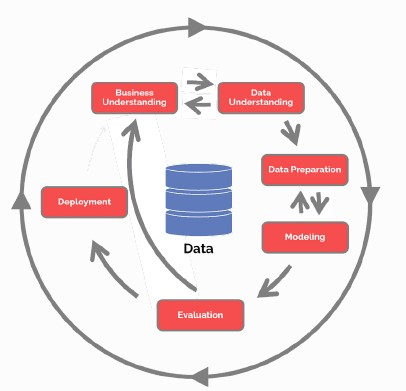
\includegraphics{images/crisp}
    \caption{\textbf{Fasi della metodologia CRISP-DM}}
    \label{fig:crisp-dm}
\end{figure}

\section{Obiettivi}\label{sec:obiettivi-daniele}
Il nostro modello Emotions Releave ha come obiettivi quelli di andare ad individuare le emozioni che più emorgono all'interno di una conversazione via chat tra persone, generando un report capace di descrivere in maniera oggettiva e imparziale cosa appare da un punto di vista esterno di quel rapporto tra quei individui.
Il nome Emotions Releave non è una scelta banale, in inglese questo termine significa "Rilascio di emozioni" ed è proprio il punto che questo progetto vuole centrare: chi usa questo tool, condividendo la sua chat, rilascia tutte le emozioni che ci sono dentri e aspetta che il tool gli risponda.
È importante sottolineare che questo modello non si pone di sostuirsi ad una figura professionale come quella dello psicologo, ma solamente essere un valido aiuto per sollevare qualche campanello d'allarme.
Per molte persone è veramente difficile accorgersi quando qualcosa non va e un punto di vista oggettivo, imparziale e pensato per questo può rappresentare uno strumento davvero utile per risolvere problemi prima che sfocino in cose più grandi, per valutare (sempre in maniera preliminare) la possibilità di appoggiarsi a professionisti o meno.
\section{Criteri di successo}\label{sec:criteri-di-successo-peas}
PEAS è l'acronimo di Performance Environment Actuators Sensor.\ È utilizzato nello studio dell'intelligenza per raggruppare in un unico termine l'ambiente operativo.
\begin{itemize}
\item \textbf{Performance} la misura di prestazione considerata prevede masssimizzare l'individuazione corretta di emozioni, data una chat in input.
\item \textbf{Environment} l'ambiente in cui opera il nostro agente è un prompt con la possibilità di inserire una chat, con una descrizione testuale (opzionale) dell'utente sul contesto.
L'ambiente risulta:
\begin{itemize}
\item \textbf{Ad agente singolo} vi sarà un unico agente singolo
\item \textbf{Parzialmente osservabile} l'agente ha visibilità di quella chat e del prompt testuale (se messo) dall'utente, in quanto non può accedere ad uno storico delle chat.
\item \textbf{Deterministico} l'ambiente rimane lo stesso, è sempre una chat con l'aggiunta di un prompt testuale
\item \textbf{Discreto} fornisce un report che dipende dal contenuto della chat
\item \textbf{Statico} è statico perché si inserisce una chat e viene fornito un report, non abbiamo dinamismo o ulteriori interazioni che fanno cambiare l'ambiente
\item \textbf{Sequenziale} le scelte fatte prima influenzeranno l'agente
\end{itemize}
\item \textbf{Actuators} l'agente agisce fornendo un report testuale (o scaricabile in formato pdf) sulla chat
\item \textbf{Sensors} l'agente agisce su testo e immagini fornite dall'utilizzatore
\end{itemize}

\section{Metriche di successo}\label{sec:metriche-di-successo}
Per valutare la qualità e il tasso di successo del modello ci affideremo a metriche come:
\begin{itemize}
    \item \textbf{Recall: } indica la capacità di catturare i veri positivi, ovvero quando effettivamente si identifica l'emozione giusta.
    \item \textbf{F1-Score: } Utile per bilanciare precisione e richiamo in scenari complessi che ci suggerisce una precisione maggiore.
\end{itemize}


\section{Organizzazione team e ruoli}\label{sec:organizzazione-team-e-ruoli}
Ogni perdsona all'interno del team ha sgli stessi ruoli,infatti l'organizzazione è team based,cioè non esiste un capo,inoltre si è deciso che prima di rendere i cambiamente effetivi di un docoumento o di publiccarlo,bisognerà fare una riunione con tutti i membri del gruppo di revisione.
\section{Analisi costi e benefici}\label{sec:analisi-costi-e-benefici}
In generale il modello si basa su un insieme di dati rappresentati da sequenze di stringhe,che sono un pò più complesse da gestire,anche nell’individuazione delle relazioni(mining) tra più sequenze(frasi) oppure correlazione tra più stringhe di una stessa sequenza.

Abbiamo scelto di basarci sul dataset "GoEmotions" , che risulta essere uno dei più completi,con tante osservazioni diverse che rappresentano le varie emozioni.La sua struttura predefinita e ben organizzata lo rende adatto agli obiettivi del nostro progetto,inoltre è distribuito gratuitamente da Google.

Per eseguire operazioni di gestione delle sequenze e magari modificarle per renderle più comprensibile al modello utilizziamo strumenti di \textbf{NLP}(Natural Language Processing).Questi strumenti permettono di eseguire operazioni di preprocessing,come normalizzazione delle frasi,rimozione ripetizioni,spelling correction ed ecc… .

Invece per individuare correlazioni (\textbf{data mining}) tra sequenze o stringhe ,usiamo dei tool kit come Pandas,utile perché include anche tecniche che realizzano la classificazione e ciò si lega bene alla risoluzione del nostro problema di classificazione.

I vari strumenti che utilizziamo,sono versioni community, per il nostro progetto realizzato non per fini aziendali,che richiedono un costo nullo,però anche se sono community offrono la maggior parte delle funzionalità che possono essere necessarie nello sviluppo delle varie fasi garantendo qualità nei risultati.

\section{Valutazioni dei rischi}\label{sec:valutazioni-dei-rischi}
Durante lo sviluppo del progetto, alcune fasi potrebbero richiedere più tempo del previsto, portando a potenziali ritardi. Un esempio significativo è la fase di Data Preparation, che comprende numerosi passaggi relativi al trattamento dei dati, come la pulizia, il pre-processing e l'organizzazione. Questa complessità è amplificata dall'ampiezza del dataset "GoEmotions", che, pur essendo un vantaggio in termini di ricchezza di informazioni, può comportare tempi più lunghi per la gestione e l'analisi.

Un ritardo nella fase di \textbf{Data Preparation} potrebbe generare un effetto domino, influenzando il completamento delle fasi successive e il rilascio finale del modello.

Un altro rischio riguarda la qualità del dataset,potrebbe verificarsi che:
\begin{itemize}
\item I dati raccolti si rivelino eccessivamente significativi ed espliciti, riducendo la variabilità necessaria per un modello robusto.
\item Oppure, i dati potrebbero risultare qualitativamente scarsi o non esaustivi rispetto agli obiettivi del progetto.
\end{itemize}
In entrambi i casi, potrebbe essere necessario selezionare un altro dataset che soddisfi meglio i requisiti del progetto, garantendo la coerenza con il modello e gli obiettivi prefissati. Questo cambio comporterebbe però un ulteriore impegno in termini di tempo e risorse.

Potremmo minimizzare l'impatto negativo di questi possibili rischi con:
\begin{itemize}
    \item \textbf{Gestione dei tempi}: Implementeremo un piano di lavoro agile, con revisioni regolari per monitorare i progressi e apportare correzioni tempestive;
    \item \textbf{Valutazione del dataset}: Fin dall'inizio verrà effettuata un'analisi approfondita della qualità e dell'adeguatezza del dataset "GoEmotions", identificando eventuali criticità;
    \item \textbf{Piani di contingenza}: Saranno individuati dataset alternativi conformi ai requisiti del progetto, pronti all'uso nel caso in cui GoEmotions si rivelasse inadeguato;
\end{itemize}

\end{document}
